%Arik Messerman, September 2006, uidarikmesserman301174 003 0021
%%% DECKBLATT ***

% Hier bitte nur ab markierten Bereich Daten �ndern

\thispagestyle{empty}
\begin{figure}[htbp]
	\centering
  \begin{minipage}[b]{41 mm}
    %
\includegraphics[width=40 mm]{AOT-Logo.png}  
    %\includegraphics[width=40 mm]{dai_logo_engl.png}
    \includegraphics[width=40 mm]{dai_logo.png}
  \end{minipage}
  %\begin{minipage}[b]{73 mm}
  % 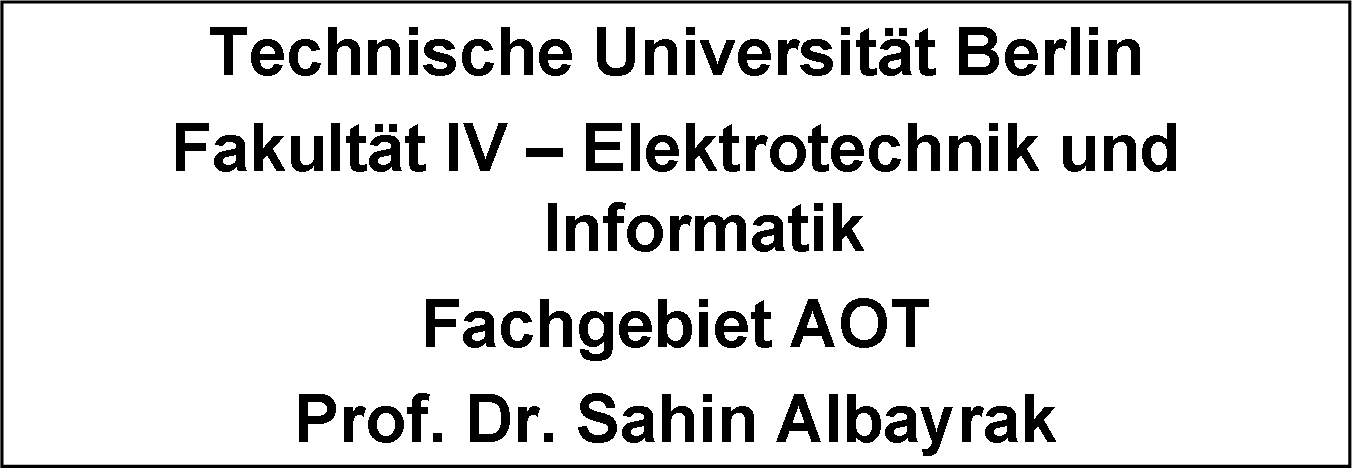
\includegraphics[width=72 mm]{figures/FakAOT2.png}  
  %\end{minipage}
	%\begin{minipage}[b]{30 mm}
  %  \includegraphics[width=30mm]{figures/TU2.png}  
  %\end{minipage}
  \label{Labelname}
\end{figure}


% Ab hier d�rfen �nderungen vorgenommen werden
\begin{center}
\begin{Huge}
Technische Universit�t Berlin\\
\vspace{1mm}
\end{Huge}{\Large Fakult�t IV - Elektrotechnik und Informatik\\
Fachgebiet AOT\\
Prof. Dr. Sahin Albayrak}\\

\vspace{26mm}
\begin{LARGE}
Dokumentenvorlage f�r einen Projektabschlussbericht\\
\end{LARGE}
\vspace{8mm}
Projekt\\
\large Sicherheit in Verteilten Umgebungen\\
\normalsize Wintersemester 2006/07\\
\vspace{4 cm}
Arik Messerman \\
Matrikel--Nummer 123456\\
\vspace{1cm}
\begin{tabular}{ll}
{\bf Betreuer} & Max Musterbetreuermann\\
\end{tabular}

\end{center}
\clearpage

